\clearpage
\VerdierPhysicalPageAnchor{0086}%
\VerdierSemanticAnchor{ch1-3-2}
\subsection{Properties of the cone functor}

\VerdierSemanticAnchor{ch1-3-2-1}
\noindent\textbf{3.2.1.}\quad
\VerdierSemanticAnchor{ch1-3-2-1-triangle-definition}
In a $\mathbb Z$-category, any diagram of the following form is called a
\emph{triangle}:

\VerdierSemanticAnchor{ch1-3-2-1-eq1}
\begin{equation}
  X\xrightarrow{u}Y\xrightarrow{v}Z\xrightarrow{w}X[1].
  \tag{3.2.1.1}
\end{equation}

\VerdierSemanticAnchor{ch1-3-2-1-notation}
To denote the triangle (3.2.1.1), we use the notation
$(X,Y,Z,u,v,w)$, or the diagram:

\VerdierSemanticAnchor{ch1-3-2-1-eq2}
\begin{equation}
  \begin{tikzpicture}[>=stealth,baseline=(current bounding box.center)]
    \node (X) at (0,0) {$X$};
    \node (Y) at (4.2,0) {$Y\mathpunct{,}$};
    \node (Z) at (2.1,1.65) {$Z$};
    \draw[->] (X) -- node[above] {$u$} (Y);
    \draw[->] (Y) -- node[right] {$v$} (Z);
    \draw[->] (Z) -- node[left] {$w$} (X);
    \draw[line width=0.45pt] (1.91,1.50) -- (1.91,1.67);
  \end{tikzpicture}
  \tag{3.2.1.2}
\end{equation}

\VerdierSemanticAnchor{ch1-3-2-1-pusher-mark}
the arrow bearing the pusher mark denoting the degree-1 morphism of the
triangle.
\VerdierSemanticAnchor{ch1-3-2-1-triangle-morphism}
Let $(X,Y,Z,u,v,w)$ and $(X',Y',Z',u',v',w')$ be two triangles. A
\emph{morphism of triangles} is a commutative diagram:

\VerdierSemanticAnchor{ch1-3-2-1-eq3}
\begin{equation}
  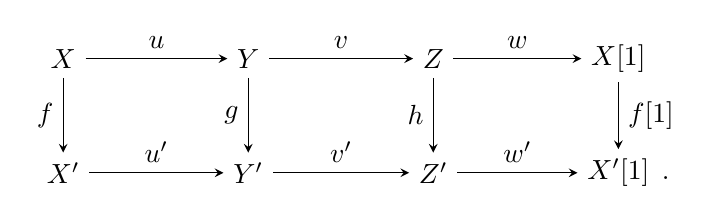
\begin{tikzpicture}[>=stealth,baseline=(current bounding box.center)]
    \node (X)  at (0,1.45) {$X$};
    \node (Y)  at (2.35,1.45) {$Y$};
    \node (Z)  at (4.70,1.45) {$Z$};
    \node (Xs) at (7.05,1.45) {$X[1]$};
    \node (Xp) at (0,0) {$X'$};
    \node (Yp) at (2.35,0) {$Y'$};
    \node (Zp) at (4.70,0) {$Z'$};
    \node (Xps) at (7.05,0) {$X'[1]$};
    \node[anchor=base west,inner sep=0pt,xshift=.08em] at (Xps.base east) {$.$};
    \draw[->] (X) -- node[above] {$u$} (Y);
    \draw[->] (Y) -- node[above] {$v$} (Z);
    \draw[->] (Z) -- node[above] {$w$} (Xs);
    \draw[->] (Xp) -- node[above] {$u'$} (Yp);
    \draw[->] (Yp) -- node[above] {$v'$} (Zp);
    \draw[->] (Zp) -- node[above] {$w'$} (Xps);
    \draw[->] (X) -- node[left] {$f$} (Xp);
    \draw[->] (Y) -- node[left] {$g$} (Yp);
    \draw[->] (Z) -- node[left] {$h$} (Zp);
    \draw[->] (Xs) -- node[right] {$f[1]$} (Xps);
  \end{tikzpicture}
  \tag{3.2.1.3}
\end{equation}

\VerdierSemanticAnchor{ch1-3-2-1-morphism-composition}
Morphisms of triangles compose in the evident way.
\VerdierSemanticAnchor{ch1-3-2-1-triangle-category}
The triangles form a category.

\VerdierSemanticAnchor{ch1-3-2-2}
\noindent\textbf{3.2.2.}\quad
\VerdierSemanticAnchor{ch1-3-2-2-source-morphism}
Let $X\xrightarrow{f}Y$ be an object of $\operatorname{tr}_1(C)$. The
following morphism (functorial in $f$) of $\operatorname{tr}_1(C)$:

\VerdierSemanticAnchor{ch1-3-2-2-eq1}
\begin{equation}
  \begin{tikzpicture}[>=stealth,baseline=(current bounding box.center)]
    \node (X)  at (0,1.35) {$X$};
    \node (Y)  at (3.6,1.35) {$Y$};
    \node (Xp) at (0,0) {$X$};
    \node (Z)  at (3.6,0) {$0$};
    \node[anchor=base west,inner sep=0pt,xshift=.08em] at (Z.base east) {$,$};
    \draw[->] (X) -- node[above] {$f$} (Y);
    \draw[->] (X) -- node[left] {$\operatorname{id}_X$} (Xp);
    \draw[->] (Y) -- (Z);
    \draw[->] (Xp) -- (Z);
  \end{tikzpicture}
  \tag{3.2.2.1}
\end{equation}

\VerdierSemanticAnchor{ch1-3-2-2-cone-application}
yields, upon applying the cone functor, a morphism of
$\operatorname{comp}(C)$, functorial in $X\xrightarrow{f}Y$, (3.1.7):

\VerdierSemanticAnchor{ch1-3-2-2-eq2}
\begin{equation}
  q(f)\colon c(f)\longrightarrow X[1].
  \tag{3.2.2.2}
\end{equation}
